% !TEX program = xelatex
% Báo cáo cải tiến: Tái sinh Di sản Số.
% Biên dịch bằng XeLaTeX (Overleaf: Menu > Compiler > XeLaTeX; tệp latexmkrc đã đặt sẵn).
% Toàn bộ báo cáo nằm trong tệp này (không chia chương thành tệp riêng).
% Phần chưa hoàn thiện được đánh dấu bằng khung vàng [CHƯA HOÀN THIỆN] (lệnh \chuahoanthien).
% Hình đặt trong thư mục figures/. Hình nào chưa có thì lệnh \hinh hiện khung vàng thay thế, đặt đúng tên tệp vào là hình tự hiện.
\documentclass[12pt,a4paper]{report}

\usepackage[a4paper,margin=2.5cm]{geometry}
\usepackage{fontspec}
\setmainfont{TeX Gyre Termes}
\setsansfont{TeX Gyre Heros}
\setmonofont{Latin Modern Mono}

\usepackage{graphicx}
\usepackage{float}
\usepackage{titlesec}
\usepackage[table]{xcolor}
\usepackage{booktabs}
\usepackage{array}
\usepackage{tabularx}
\usepackage{enumitem}
\usepackage{caption}
\usepackage{amsmath}
\usepackage{pgfplots}
\pgfplotsset{compat=1.17}
\usepackage[colorlinks=true,linkcolor=blue!50!black,urlcolor=blue!50!black,citecolor=blue!50!black]{hyperref}

% Tiếng Việt: không ngắt từ bằng gạch nối (mỗi âm tiết đã là một từ), giãn dòng vừa phải
\hyphenpenalty=10000
\exhyphenpenalty=10000
\sloppy
\emergencystretch=2em
\linespread{1.12}
\setlength{\parskip}{4pt}
\setlength{\parindent}{0pt}
\setlist{itemsep=2pt,topsep=3pt,parsep=0pt}
\captionsetup{font=small,labelfont=bf}
\renewcommand{\topfraction}{0.9}
\renewcommand{\bottomfraction}{0.8}
\renewcommand{\textfraction}{0.1}
\renewcommand{\floatpagefraction}{0.8}
\setlength{\textfloatsep}{8pt plus 2pt minus 2pt}
\setlength{\intextsep}{7pt plus 2pt minus 2pt}
\setlength{\floatsep}{7pt plus 2pt minus 2pt}
\renewcommand{\arraystretch}{1.15}

% Tên các mục theo tiếng Việt
\renewcommand{\chaptername}{}
\renewcommand{\contentsname}{Mục lục}
\renewcommand{\listfigurename}{Danh mục hình}
\renewcommand{\listtablename}{Danh mục bảng}
\renewcommand{\figurename}{Hình}
\renewcommand{\tablename}{Bảng}
\renewcommand{\appendixname}{Phụ lục}
\renewcommand{\bibname}{Tài liệu tham khảo}
\titleclass{\chapter}{straight}
\titleformat{\chapter}[hang]{\LARGE\bfseries}{\thechapter.}{0.6em}{}
\titleformat{\section}[hang]{\Large\bfseries}{\thesection}{0.6em}{}
\titlespacing*{\chapter}{0pt}{28pt}{24pt}

% Khung vàng đánh dấu phần chưa hoàn thiện hoặc cần nhóm điền
\newcommand{\chuahoanthien}[1]{%
  \par\medskip\noindent\colorbox{yellow!30}{\parbox{\dimexpr\linewidth-2\fboxsep\relax}{\small\textbf{[CHƯA HOÀN THIỆN]} #1}}\par\medskip}

% Chèn hình: \hinh{đường dẫn trong figures/}{độ rộng}{chú thích}{nhãn}. Thiếu tệp thì hiện khung vàng.
\newcommand{\hinh}[4]{%
  \IfFileExists{figures/#1}%
    {\begin{figure}[H]\centering\includegraphics[width=#2]{figures/#1}\caption{#3}\label{#4}\end{figure}}%
    {\chuahoanthien{Chưa có hình \ma{figures/#1}. Nội dung hình: #3}}}

% Hình rộng hơn khổ chữ một chút (sơ đồ nhiều chữ nhỏ)
\newcommand{\hinhrong}[3]{%
  \IfFileExists{figures/#1}%
    {\begin{figure}[H]\centering\makebox[\textwidth][c]{\includegraphics[width=1.15\textwidth]{figures/#1}}\caption{#2}\label{#3}\end{figure}}%
    {\chuahoanthien{Chưa có hình \ma{figures/#1}. Nội dung hình: #2}}}

% Ảnh ngang giữ nguyên chiều, giới hạn trong khổ trang dọc
\newcommand{\hinhngang}[3]{%
  \IfFileExists{figures/#1}%
    {\begin{figure}[H]\centering\includegraphics[width=\textwidth,height=0.82\textheight,keepaspectratio]{figures/#1}\caption{#2}\label{#3}\end{figure}}%
    {\chuahoanthien{Chưa có hình \ma{figures/#1}. Nội dung hình: #2}}}

% Hình cao (sơ đồ BPMN dọc): một trang riêng, chiều cao tối đa gần hết trang
\newcommand{\hinhcao}[3]{%
  \IfFileExists{figures/#1}%
    {\begin{figure}[H]\centering\includegraphics[width=\textwidth,height=0.9\textheight,keepaspectratio]{figures/#1}\caption{#2}\label{#3}\end{figure}}%
    {\chuahoanthien{Chưa có hình \ma{figures/#1}. Nội dung hình: #2}}}

% Tên chỉ số và mã nguồn: chữ đơn cách, cho phép ngắt dòng ở dấu gạch dưới
\newcommand{\ma}[1]{\texttt{\detokenize{#1}}}

\begin{document}

\begin{titlepage}
% Viền xanh dương đậm quanh trang bìa: một nét dày ngoài, một nét mảnh trong.
% Cần biên dịch hai lần để tikz định vị đúng trang (Overleaf tự làm).
\definecolor{vienbia}{RGB}{0,45,120}
\begin{tikzpicture}[remember picture,overlay]
  \draw[line width=3.5pt,color=vienbia]
    ([xshift=1.2cm,yshift=-1.2cm]current page.north west) rectangle
    ([xshift=-1.2cm,yshift=1.2cm]current page.south east);
  \draw[line width=0.8pt,color=vienbia]
    ([xshift=1.5cm,yshift=-1.5cm]current page.north west) rectangle
    ([xshift=-1.5cm,yshift=1.5cm]current page.south east);
\end{tikzpicture}
\centering
\vspace*{2cm}
{\large Cuộc thi Sáng tạo trẻ Quốc gia trong lĩnh vực Trí tuệ nhân tạo năm 2026\par}
\vspace{2.5cm}
{\Huge\bfseries BÁO CÁO CẢI TIẾN\par}
\vspace{0.8cm}
{\Large\bfseries Dự án Tái sinh Di sản Số\par}
\vspace{0.4cm}
{\large Sinh hoa văn gốm Bát Tràng lên áo dài bằng trí tuệ nhân tạo\par}
\vspace{3cm}
% Thông tin đội thi
{\large\textbf{Tên đội thi:} 3 chàng hiệp sĩ mộng mơ \qquad \textbf{Mã đội:} AI26C0005\par}
\vspace{0.6cm}
\begin{tabular}{@{}>{\raggedright\arraybackslash}p{2.6cm}>{\raggedright\arraybackslash}p{4.4cm}>{\raggedright\arraybackslash}p{7.2cm}@{}}
\toprule
\textbf{Thành viên} & \textbf{Họ và tên} & \textbf{Đơn vị} \\
\midrule
Thành viên 1 & Đồng Tiến Đoàn & Trường Đại học Kinh tế - Luật, ĐHQG HCM \\
Thành viên 2 & Vương Anh Kiệt & Trường Đại học Kinh tế - Luật, ĐHQG HCM \\
Thành viên 3 & Trịnh Hữu Kiến Quốc & Trường Đại học Công thương TP.HCM \\
\bottomrule
\end{tabular}
\vfill
{\large Tháng 11 năm 2026\par}
\end{titlepage}

\tableofcontents
\clearpage
\listoffigures
\clearpage

%==============================================================================
% TÓM TẮT
%==============================================================================
\chapter*{Tóm tắt}
\addcontentsline{toc}{chapter}{Tóm tắt}

Hệ thống Tái sinh Di sản Số đưa hoa văn trên gốm men lam Bát Tràng lên áo dài. Báo cáo này trình bày các cải tiến của hệ thống theo ba yêu cầu cải tiến. Hệ thống đã có bằng chứng kỹ thuật cho cả ba yêu cầu. Nội dung còn thiếu là phiếu nhận xét, đánh giá của người am hiểu di sản vì nhóm chưa liên hệ được.

\begin{table}[H]
\centering
\setlength{\tabcolsep}{4pt}
\footnotesize
\caption{Tóm tắt ba yêu cầu của ban tổ chức, phần đã làm và phần còn thiếu.}
\label{tab:tomtat}
\begin{tabularx}{\textwidth}{>{\raggedright\arraybackslash}p{3.3cm}>{\raggedright\arraybackslash}X>{\raggedright\arraybackslash}p{4.2cm}}
\toprule
\textbf{Yêu cầu cải tiến} & \textbf{Đã thực hiện} & \textbf{Hạn chế còn lại} \\
\midrule
1. Đánh giá thiết kế cuối, không chỉ hoa văn trung gian &
Hai cổng chất lượng: G2 cho hoa văn, G3 cho thiết kế cuối với năm chỉ số. Hoàn thiện ảnh chỉ trong vùng áo, có khóa họa tiết. Vòng loại và thử lại tối đa 3 lần. &
Chưa liên hệ được với người am hiểu di sản để xin nhận xét, đánh giá \\
\addlinespace
2. Đối chứng có kiểm soát, nhiều seed, chấm mù &
Chạy thực nghiệm 120 lượt với 5 seed. Có bảng điểm do 28 người chấm mù (chọn 2 seed + thay trọng số ControlNet để chấm) &
\textit{Đã hoàn thành} \\
\addlinespace
3. Nguồn gốc, bản quyền, truy vết &
Nguồn và giấy phép CC BY 4.0 cho 6 hiện vật. Design Passport có chuỗi mã băm, kiểm toàn vẹn đạt 28/28. Nhãn “Hỗ trợ bởi AI”. Lịch sử sửa thủ công đã kiểm tra và đạt yêu cầu &
\textit{Đã hoàn thành} \\
\bottomrule
\end{tabularx}
\end{table}



%==============================================================================
% CHƯƠNG 1. BỐI CẢNH VÀ MỤC TIÊU
%==============================================================================
\chapter{Bối cảnh và mục tiêu}

\section{Bài toán}

Gốm men lam Bát Tràng có hệ hoa văn phong phú: dây hoa, mẫu đơn, rồng mây, huy hiệu. Hệ thống Tái sinh Di sản Số biến những hoa văn này thành thiết kế áo dài. Người dùng chọn một hiện vật số hóa. Hệ thống trả về bốn thiết kế áo dài, ứng với bốn mức sáng tạo, trong đó họa tiết gốm được giữ nhận ra được và dáng áo không bị biến dạng.

Đầu vào của mô hình sinh là \emph{mảng hoa văn phẳng}, tức texture UV trải phẳng của mô hình 3D hiện vật, cạnh dài khoảng 2.048 điểm ảnh. Ảnh render cả bình chỉ dùng để hiển thị và nhận diện. Quy trình sinh ảnh có hai giai đoạn và được cải tiến thêm so với quy trình cũ:
\begin{enumerate}
  \item Stable Diffusion 1.5 kết hợp ControlNet Canny sinh \emph{hoa văn phẳng} từ mảng hoa văn gốc \cite{rombach2022,zhang2023controlnet}.
  \item Hoa văn được \emph{ghép tất định} lên một chiếc áo dài nền do LoRA sinh ra \cite{hu2021lora}. Mô hình SAM tách vùng áo \cite{kirillov2023sam}, CLIP chọn bố cục họa tiết trên áo \cite{radford2021clip}, rồi một bước hoàn thiện img2img chỉ chạy trong vùng áo, có khóa họa tiết.
\end{enumerate}



\section{Ba yêu cầu cải tiến}

Ba yêu cầu cải tiến tương ứng của dự án:
\begin{enumerate}
  \item \textbf{Đánh giá thiết kế cuối.} Hệ thống phải đo chất lượng của thiết kế áo dài cuối cùng, không chỉ hoa văn trung gian. Ngoài ra, cần có nhận xét từ người am hiểu về di sản.
  \item \textbf{Đối chứng có kiểm soát.} Thí nghiệm phải đổi từng yếu tố một, thử nhiều seed và chấm mù. Có bảng điểm do người đánh giá.
  \item \textbf{Nguồn gốc, bản quyền, truy vết.} Hệ thống phải ghi nguồn và giấy phép hiện vật, ghi công, lịch sử biên tập thủ công và nhãn nội dung có hỗ trợ AI.
\end{enumerate}

\section{Hạn chế của hệ thống cũ}

Trước khi cải tiến, nhóm rà soát lại hệ thống cũ và ghi nhận các hạn chế sau tương ứng với từng yêu cầu cải tiến.

\begin{table}[H]
\centering
\small
\caption{Hạn chế của hệ thống cũ và yêu cầu cải tiến tương ứng.}
\label{tab:hanche}
\begin{tabularx}{\textwidth}{>{\raggedright\arraybackslash}p{3.2cm}>{\raggedright\arraybackslash}X>{\raggedright\arraybackslash}p{3.0cm}}
\toprule
\textbf{Hiện trạng} & \textbf{Hệ quả} & \textbf{Yêu cầu liên quan} \\
\midrule
Chỉ đo hoa văn trung gian (độ tương đồng CLIP). Thiết kế áo dài cuối không được đo &
Không biết bước img2img có phá họa tiết hay dáng áo dài hay không & Yêu cầu 1 \\
Bước img2img độ nhiễu 0,40 chạy trên toàn ảnh, không kiểm tra sau đó &
Đo lại 24 thiết kế cũ cho thấy 20 thiết kế có điểm giữ họa tiết (PPS) dưới 0,40, tức họa tiết bị vẽ lại quá nhiều & Yêu cầu 1 \\
Bốn biến thể đổi cùng lúc bốn yếu tố, chỉ chạy một seed &
Không quy được khác biệt cho yếu tố nào, không biết độ dao động theo seed & Yêu cầu 2 \\
6 hiện vật chưa có sự cho phép sử dụng & Dữ liệu có nguy cơ không được phép sử dụng miễn phí, vi phạm đạo đức dữ liệu & Yêu cầu 3 \\
Design Passport chỉ có 4 trường, không có phiên bản, lịch sử chỉnh sửa, phê duyệt hay nhãn AI &
Không chứng minh được thiết kế đi từ nguồn nào, ai sửa gì & Yêu cầu 3 \\
\bottomrule
\end{tabularx}
\end{table}

\section{Bảng so sánh trước và sau cải tiến}

\begin{table}[H]
\centering
\small
\caption{So sánh trước và sau cải tiến.}
\label{tab:truocsau}
\begin{tabularx}{\textwidth}{>{\raggedright\arraybackslash}p{3.0cm}>{\raggedright\arraybackslash}X>{\raggedright\arraybackslash}X>{\raggedright\arraybackslash}p{1.6cm}}
\toprule
\textbf{Nội dung} & \textbf{Hệ thống cũ} & \textbf{Bản cải tiến} & \textbf{Chương} \\
\midrule
Đánh giá chất lượng & Độ tương đồng CLIP của hoa văn trung gian & Cổng G2 (hoa văn) và G3 (thiết kế cuối, năm chỉ số) & 3 \\
Hoàn thiện ảnh & img2img toàn ảnh, độ nhiễu 0,40, không kiểm sau đó & Chỉ trong vùng áo, độ nhiễu 0,20, khóa họa tiết, vòng loại và thử lại & 3 \\
Thí nghiệm & Bốn biến thể đổi bốn yếu tố, một seed & Thí nghiệm trên nhiều seed và trọng số ControlNet, thiết lập gói chấm mù có người đánh giá, thống kê kết quả dao động & 4 \\
Truy vết & Ghi đè ảnh cũ, Passport chỉ có 4 trường & Mỗi lần chạy sinh kết quả tại một thư mục riêng, Passport có phiên bản, nhật ký thiết kế có mã băm, nhãn AI & 5 \\
Người tham gia và chỉnh sửa ảnh & Không có & Tải bản sửa lên, chạy lại cổng kiểm tra chất lượng, ghi vào Passport & 5 \\
\bottomrule
\end{tabularx}
\end{table}

%==============================================================================
% CHƯƠNG 2. PIPELINE AI SINH ẢNH THIẾT KẾ
%==============================================================================
\chapter{Pipeline AI sinh ảnh thiết kế}



Bốn thiết kế trong các hình có bốn mức sáng tạo, từ trái sang phải; mức càng cao thì trọng số ControlNet càng thấp (0,85; 0,65; 0,45; 0,25).

\section{Chuẩn bị đầu vào (bước 1 đến 4)}

\textbf{Bước 1. Hiện vật gốc.} Ảnh render cả bình từ mô hình 3D, dùng để hiển thị và nhận diện, không dùng làm đầu vào cho mô hình.

\textbf{Bước 2. Mảng hoa văn phẳng.} Texture UV trải phẳng của mô hình 3D có sẵn trong bộ dữ liệu, là đầu vào chính của mô hình sinh. Hệ thống cắt vùng đảo UV có nhiều nét mực lam nhất.

\textbf{Bước 3. Ảnh tham chiếu.} Phần được cắt từ mảng phẳng, đưa về khung vuông 512 điểm ảnh.

\textbf{Bước 4. Ảnh Canny điều khiển.} Bản đồ cạnh Canny chỉ giữ nét hoa văn, bỏ nét viền bình, để ControlNet bám theo hoa văn thay vì dáng bình.

\begin{figure}[H]
\centering
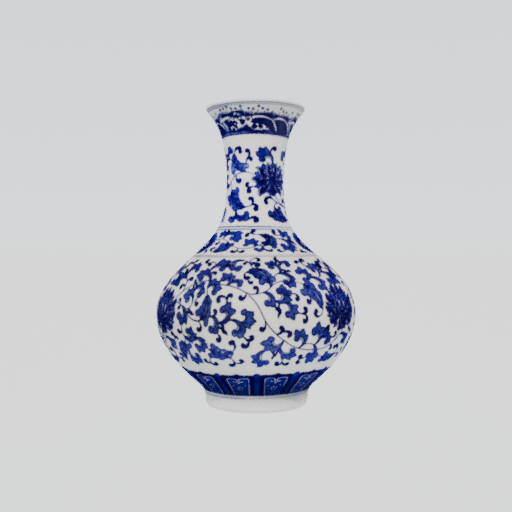
\includegraphics[height=3.6cm]{figures/pipeline/buoc01_hien_vat_goc.png}\hfill
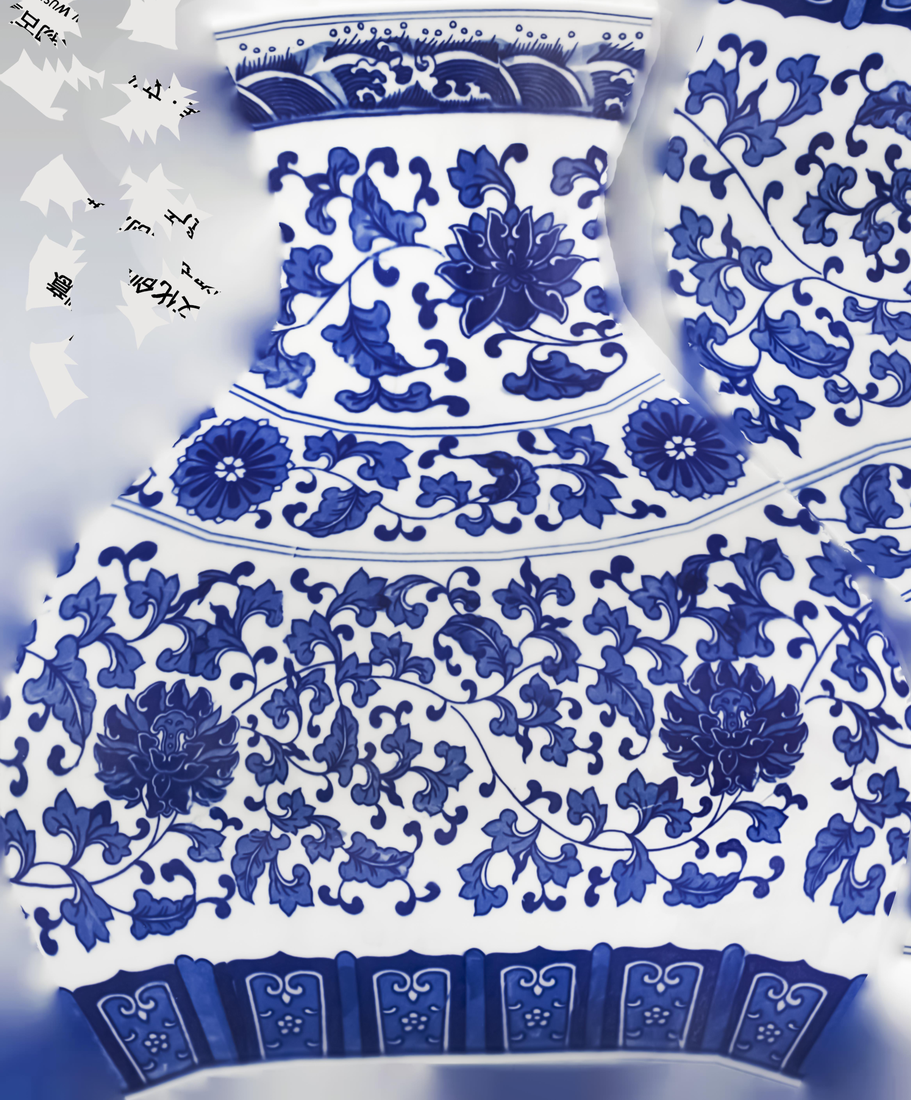
\includegraphics[height=3.6cm]{figures/pipeline/buoc02_panel_texture_trai_phang.png}\hfill
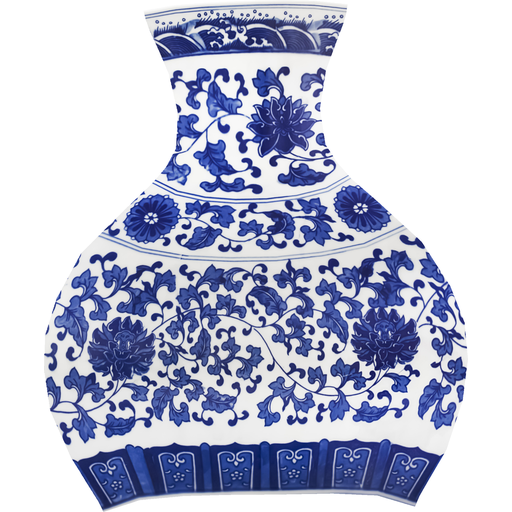
\includegraphics[height=3.6cm]{figures/pipeline/buoc03_anh_tham_chieu.png}\hfill
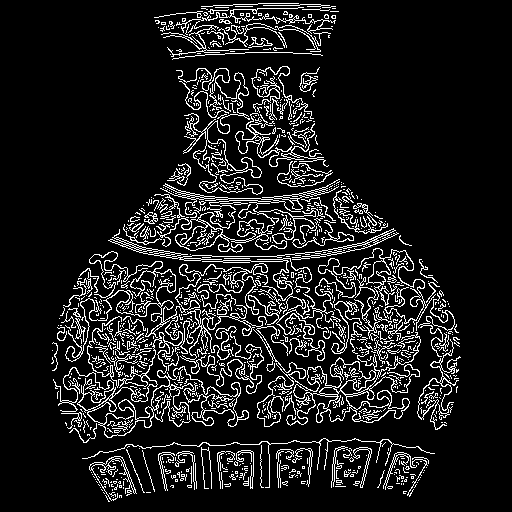
\includegraphics[height=3.6cm]{figures/pipeline/buoc04_anh_canny_dieu_khien.png}
\caption{Bước 1 đến 4, từ trái sang phải: hiện vật gốc, mảng hoa văn phẳng, ảnh tham chiếu, ảnh Canny điều khiển.}
\label{fig:pl14}
\end{figure}

\section{Sinh hoa văn và áo dài nền (bước 5 và 6)}

\textbf{Bước 5. Hoa văn sinh ra, bốn mức.} Stable Diffusion 1.5 kết hợp ControlNet Canny sinh hoa văn phẳng. Trọng số ControlNet càng thấp thì hoa văn càng tự do so với ảnh gốc. Hoa văn đi qua cổng G2 (mục \ref{sec:g2}).

\hinh{pipeline/buoc05_hoa_van_sinh_ra_4_muc.png}{\textwidth}{Bước 5: bốn hoa văn phẳng ứng với bốn mức trọng số ControlNet.}{fig:pl5}

\textbf{Bước 6. Áo dài nền.} Một áo dài trắng do mô hình Stable Diffusion kèm LoRA dáng áo dài sinh ra. LoRA được huấn luyện từ bộ ảnh VietFashion \cite{cao2026vietfashion}. Giấy phép của bộ ảnh này là CC BY-NC 4.0 nên hệ thống bị ràng buộc \emph{chỉ dùng phi thương mại} (xem mục \ref{sec:rights}).

\textbf{Bước 7. Vùng áo.} Mô hình SAM tách vùng áo khỏi nền; hình tô đỏ vùng được chọn.

\begin{figure}[H]
\centering
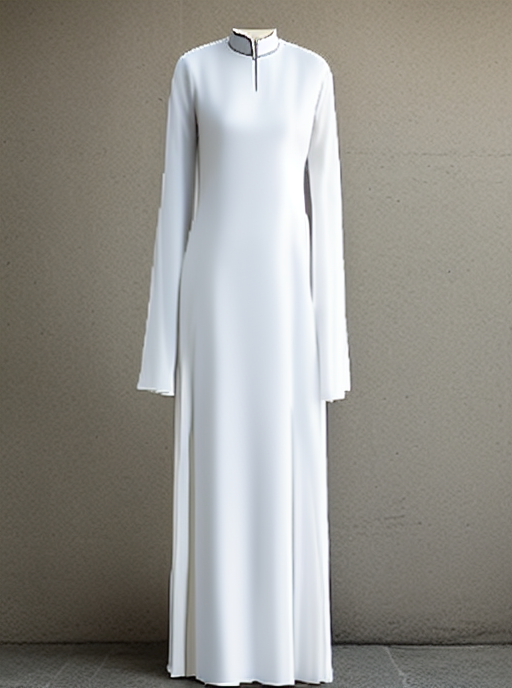
\includegraphics[height=5.2cm]{figures/pipeline/buoc06_ao_dai_nen_lora.png}\hspace{1cm}
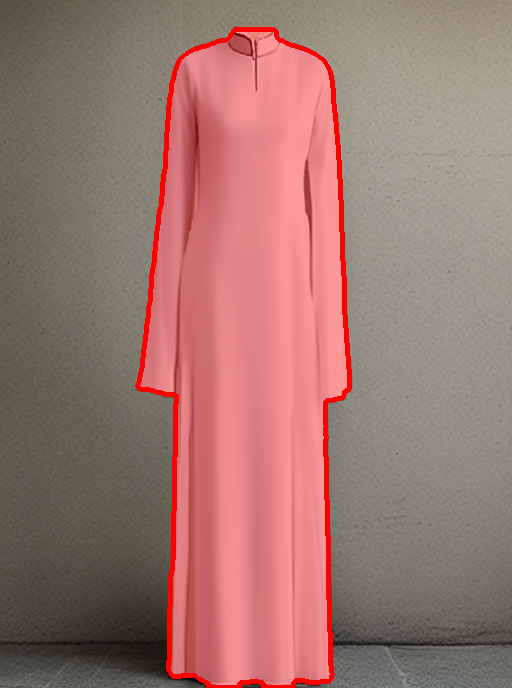
\includegraphics[height=5.2cm]{figures/pipeline/buoc07_vung_ao_sam_to_do.png}
\caption{Bước 6 và 7: áo dài nền do LoRA sinh (trái) và vùng áo do SAM tách, tô đỏ (phải).}
\label{fig:pl67}
\end{figure}

\section{Chọn bố cục và ghép (bước 8 đến 10)}

\textbf{Bước 8. Mask vùng in.} Với mỗi thiết kế, CLIP xếp hạng bảy bố cục họa tiết trên áo (ví dụ dải thân trước, bảng gấu tà) và chọn một. Vùng in là phần giao của vùng bố cục (hình siêu elip có mép mềm) với mask áo đã co lại và làm mờ mép. Nhờ giao với mask áo, họa tiết không lem ra ngoài áo.

\textbf{Bước 9. Vùng in tô đỏ.} Hình tô đỏ phần vùng in thật sự, để kiểm tra bằng mắt rằng hoa văn nằm trong áo.

\textbf{Bước 10. Ghép thô.} Hoa văn được ghép \emph{tất định} lên áo nền (mask mềm, độ dịch chuyển theo nếp vải, đổ bóng). Bản ghép thô đúng tuyệt đối về dáng áo và vị trí họa tiết, và là mốc so sánh cho cổng G3 (mục \ref{sec:g3}).

\hinh{pipeline/buoc08_mat_na_vung_in_4_bo_cuc.png}{\textwidth}{Bước 8: mask vùng in của bốn bố cục.}{fig:pl8}
\hinh{pipeline/buoc09_vung_in_to_do_4_bo_cuc.png}{\textwidth}{Bước 9: vùng in tô đỏ trên áo, bốn bố cục.}{fig:pl9}
\hinh{pipeline/buoc10_ghep_hoa_van_len_ao_tho_4_bo_cuc.png}{\textwidth}{Bước 10: bản ghép thô, bốn bố cục.}{fig:pl10}

\section{Hoàn thiện (bước 11)}

\textbf{Bước 11. Kết quả sau hoàn thiện.} Một lượt img2img độ nhiễu 0,20 chỉ chạy trong vùng áo, làm mềm vải và ánh sáng. Sau đó \emph{khóa họa tiết} trả lại nét vẽ và màu họa tiết từ bản ghép thô, phần ánh sáng và bóng vải lấy từ bước hoàn thiện. Kết quả đi qua cổng G3 (mục \ref{sec:g3}).

\hinh{pipeline/buoc11_ket_qua_sau_polish_4_thiet_ke.png}{\textwidth}{Bước 11: bốn thiết kế cuối sau hoàn thiện.}{fig:pl11}

%==============================================================================
% CHƯƠNG 3. CẢI TIẾN 1 (YÊU CẦU 1)
%==============================================================================
\chapter{Cải tiến 1: đánh giá thiết kế cuối}


\section{Nguyên tắc}

Hệ thống chỉ đo \emph{kỹ thuật}. Kết quả đo chỉ quyết định thiết kế \emph{đủ điều kiện chuyển chuyên gia thẩm định} hay \emph{phải sửa, sinh lại}. Không chỉ số nào tự phê duyệt thiết kế; văn hóa và thẩm mỹ do chuyên gia quyết định.

Các ảnh dùng để đo trong một thiết kế:
\begin{itemize}
  \item \emph{reference}: ảnh hiện vật đã đưa về khung 512 điểm ảnh, đầu vào của giai đoạn 1;
  \item \emph{pattern}: hoa văn phẳng do SD1.5 và ControlNet sinh ra;
  \item \emph{raw}: bản ghép tất định hoa văn lên áo (trước hoàn thiện);
  \item \emph{final}: thiết kế cuối sau hoàn thiện img2img;
  \item \emph{template}: ảnh áo dài trắng nền.
\end{itemize}
Cổng G3 so \emph{final} với \emph{raw} vì \emph{raw} đúng tuyệt đối về dáng áo và vị trí họa tiết. Mọi khác biệt từ \emph{raw} sang \emph{final} đều do bước hoàn thiện gây ra, sau img2img toàn ảnh, dáng áo và hoa văn gốc có thể bị biến dạng.

\section{Cổng G2: chất lượng hoa văn}
\label{sec:g2}

G2 đo hoa văn phẳng ngay sau giai đoạn 1, trước khi đưa lên áo.

\textbf{Rò dáng vật chứa} (\ma{vessel_leakage}, viết tắt VLS). Lỗi nhóm đã phát hiện khi thực nghiệm: ở trọng số ControlNet cao, có một số lượt “hoa văn” sinh ra là ảnh nguyên chiếc bình trên nền trơn. Việc này dẫn đến thay vì chỉ in hoa văn lên áo thì in nguyên chiếc bình. Một ô hoa văn đúng nghĩa phải phủ kín khung. Vì vậy chỉ số đánh giá được chọn cho là điểm khi nhân hai đại lượng: tỉ lệ viền khung (rộng 24 điểm ảnh) là nền trơn, và IoU giữa dáng vật thể trong hoa văn với dáng hiện vật gốc. Cả hai cùng cao nghĩa là thay vì hoa văn thì mô hình đang vẽ lại cả cái bình.
\[
\mathrm{VLS}=r_{\text{viền nền trơn}}\times \mathrm{IoU}(M_{\text{hoa văn}},M_{\text{hiện vật}})
\]

\textbf{Đường nối khi lát} (\ma{seam_ratio}). Hoa văn được lát nhiều lần trên áo, nên mép trái phải và trên dưới phải liền mạch. Chỉ số này là chênh lệch trung bình giữa hai mép đối diện, chia cho chênh lệch trung bình giữa hai cột (hàng) kề nhau bên trong ảnh, lấy giá trị lớn hơn theo hai chiều. Giá trị gần 1 là liền mạch.
\[
h=\frac{\overline{|g_{:,0}-g_{:,W-1}|}}{\overline{|\Delta_x g|}},\qquad
v=\frac{\overline{|g_{0,:}-g_{H-1,:}|}}{\overline{|\Delta_y g|}},\qquad
\mathrm{seam}=\max(h,v)
\]
Ở đây $g$ là ảnh xám của ô hoa văn, cao $H$ và rộng $W$ điểm ảnh. $g_{:,0}$ và $g_{:,W-1}$ là cột đầu và cột cuối, $g_{0,:}$ và $g_{H-1,:}$ là hàng đầu và hàng cuối. $\Delta_x g$ và $\Delta_y g$ là hiệu giữa hai cột kề nhau và giữa hai hàng kề nhau. Thanh ngang trên đầu là lấy trung bình. $h$ đo đường nối trái phải, $v$ đo đường nối trên dưới.

\section{Cổng G3: chất lượng thiết kế cuối}
\label{sec:g3}

G3 gồm năm chỉ số có ngưỡng. Một số chỉ số chỉ tính trong \emph{vùng họa tiết}, tức các điểm ảnh nằm trong vùng in của bố cục và khác áo trắng nền rõ rệt (sai khác màu $\Delta E_{76}>8$). Nếu tính trên cả vùng in, phần vải trắng giữ nguyên sẽ làm điểm cao giả.

Các ký hiệu màu dùng trong cổng này thuộc không gian màu CIELAB (gọi tắt là Lab), tách màu thành ba kênh. $L^*$ là độ sáng, từ 0 (đen) đến 100 (trắng). $a^*$ là trục xanh lá với đỏ: âm là xanh lá, dương là đỏ. $b^*$ là trục xanh dương với vàng: âm là xanh dương, dương là vàng. Hai kênh $a^*$, $b^*$ cho biết sắc độ (màu gì), không phụ thuộc sáng tối. Màu trắng, xám, đen có $a^*$ và $b^*$ gần 0. $\Delta E_{76}$ là sai khác giữa hai màu, tính bằng khoảng cách Euclid trong Lab:
\[
\Delta E_{76}=\sqrt{(L_1^*-L_2^*)^2+(a_1^*-a_2^*)^2+(b_1^*-b_2^*)^2}
\]
Giá trị càng lớn thì hai màu càng khác nhau.

\textbf{Giữ họa tiết} (PPS, \ma{pattern_preservation}). Đây là chỉ số chính cho yêu cầu cải tiến 1. PPS là trung bình của hai hệ số tương quan chuẩn hóa (NCC) trong vùng họa tiết, sau khi căn \emph{final} về \emph{raw} bằng ECC: tương quan nét vẽ, tính trên dải tần trung của kênh sáng $L^*$ (hiệu hai bộ lọc Gauss, $\sigma=1{,}2$ và $4{,}0$, giữ nét vẽ họa tiết, bỏ bóng nếp vải và nhiễu hạt), và tương quan sắc độ, tính trên hai kênh màu $a^*$ và $b^*$.
\[
\begin{aligned}
\mathrm{NCC}(a,b) &= \frac{\sum (a-\bar a)(b-\bar b)}{\sqrt{\sum (a-\bar a)^2\;\sum (b-\bar b)^2}}, \\
\mathrm{PPS} &= \tfrac12\big(\mathrm{NCC}_{\text{nét vẽ}}+\mathrm{NCC}_{\text{sắc độ}}\big), \\
\mathrm{NCC}_{\text{sắc độ}} &= \tfrac12\Big(\mathrm{NCC}(a^*_{\text{raw}},a^*_{\text{final}})+\mathrm{NCC}(b^*_{\text{raw}},b^*_{\text{final}})\Big).
\end{aligned}
\]

Hệ số NCC (normalized cross-correlation) là hệ số tương quan $r$, nên bình phương của nó là tỉ lệ phương sai giải thích được. Với tương quan nét vẽ: $r=0{,}6$ nghĩa là khoảng 36\% phương sai nét vẽ của bản ghép còn giải thích được trong thiết kế cuối; $r<0{,}4$ nghĩa là dưới 16\%, tức họa tiết đã bị vẽ lại. Cách diễn giải này đúng cho riêng thành phần nét vẽ. PPS là trung bình của hai thành phần nên chỉ là điểm tổng hợp, không phải một hệ số tương quan.

\textbf{Giữ dáng áo} (\ma{garment_shape_iou}, GSC). Dáng áo của \emph{raw} và \emph{final} được tách bằng GrabCut, khởi tạo từ mask áo (lõi chắc chắn là áo, vành là có thể là áo, xa hơn là nền), rồi tính IoU. IoU dưới 0,92 tương đương lệch từ 8\% diện tích áo.
\[
\mathrm{GSC}=\frac{|S_{\text{raw}}\cap S_{\text{final}}|}{|S_{\text{raw}}\cup S_{\text{final}}|}
\]

\textbf{Độ nét} (\ma{sharpness_ratio}) và \textbf{giữ chi tiết mịn} (\ma{detail_ratio}). Cả hai là tỉ số phương sai Laplacian của \emph{final} trên \emph{raw}. Độ nét đo trong cả vùng áo. Chi tiết mịn đo riêng trong vùng họa tiết, nên bắt được việc nét mảnh bị nhòe sau hoàn thiện, điều mà PPS (chỉ đo dải tần trung) không thấy.
\[
\mathrm{ratio}=\frac{\mathrm{Var}\big[\nabla^2 I_{\text{final}}\big]_{R}}{\mathrm{Var}\big[\nabla^2 I_{\text{raw}}\big]_{R}}
\]
Ở đây $I$ là ảnh xám, $\nabla^2 I$ là Laplacian của $I$ (đạo hàm bậc hai theo hai hướng, lớn ở nét sắc), và $R$ là vùng đo: vùng áo cho độ nét, vùng họa tiết cho chi tiết mịn.

\textbf{Lệch bảng màu} (\ma{palette_shift_de}). Khoảng cách màu $\Delta E_{76}$ giữa màu trung bình của vùng họa tiết ở hai ảnh trong không gian Lab. $\Delta E\approx 10$ là khác màu nhìn rõ khi đặt cạnh nhau.


\section{Ngưỡng và quyết định}

\begin{table}[H]
\centering
\small
\caption{Ngưỡng của hai cổng chất lượng do nhóm chọn.}
\label{tab:nguong}
\begin{tabularx}{\textwidth}{>{\raggedright\arraybackslash}p{1.6cm}>{\raggedright\arraybackslash}X>{\centering\arraybackslash}p{1.9cm}>{\centering\arraybackslash}p{1.6cm}>{\raggedright\arraybackslash}p{2.0cm}}
\toprule
\textbf{Cổng} & \textbf{Chỉ số} & \textbf{Cảnh báo} & \textbf{Loại} & \textbf{Chiều tốt} \\
\midrule
G2 & Rò dáng vật chứa (VLS) & từ 0,20 & từ 0,40 & thấp \\
G2 & Đường nối khi lát & từ 1,5 & từ 2,0 & thấp \\
G3 & Giữ họa tiết (PPS) & dưới 0,60 & dưới 0,40 & cao \\
G3 & Giữ dáng áo (IoU) & dưới 0,95 & dưới 0,92 & cao \\
G3 & Độ nét so với bản ghép & dưới 0,45 & dưới 0,25 & cao \\
G3 & Giữ chi tiết mịn & dưới 0,85 & dưới 0,60 & cao \\
G3 & Lệch bảng màu ($\Delta E$) & từ 10 & từ 20 & thấp \\
\bottomrule
\end{tabularx}
\end{table}

Mỗi chỉ số được xếp PASS, WARN hoặc FAIL theo ngưỡng. Quyết định của cổng lấy mức tệ nhất trong các chỉ số của cổng đó. Quyết định chung của thiết kế như sau:
\begin{itemize}
  \item G2 hoặc G3 \textbf{FAIL}: không chuyển chuyên gia, hệ thống đề xuất bước quay lại cụ thể;
  \item \textbf{WARN}: người kiểm soát chất lượng (QC) xem xét trước khi chuyển chuyên gia, có thể kèm ghi chú;
  \item \textbf{PASS}: đủ điều kiện chuyển chuyên gia thẩm định.
\end{itemize}

\textbf{Vòng loại và thử lại.} Khi G2 không đạt, hệ thống sinh lại hoa văn với seed kế tiếp hoặc giảm một mức trọng số ControlNet, giữ nguyên prompt và bảng màu. Khi G3 không đạt, hệ thống thử hoàn thiện lại bằng khóa họa tiết hoặc giảm độ nhiễu img2img (từ 0,40 xuống 0,25); nếu vẫn không đạt thì dùng bản ghép tất định, vì bản này đúng tuyệt đối về dáng áo. Mỗi thiết kế được thử lại tối đa 3 lần; quá 3 lần thì chuyển nhà thiết kế quyết định.

\textbf{Hoàn thiện có kiểm soát.} Khác bản trước (img2img toàn ảnh, độ nhiễu 0,40), bản cải tiến chạy img2img độ nhiễu 0,20 \emph{chỉ trong vùng áo}, rồi áp khóa họa tiết: trả lại nét vẽ và màu họa tiết từ bản ghép thô, còn ánh sáng và bóng vải lấy từ bước hoàn thiện.

\hinh{passport/lan1/passport_6_chat_luong.png}{1.0\textwidth}{Phần \texttt{quality} của một Design Passport (thiết kế ví dụ, trước khi sửa tay), chia ba đoạn. Cổng G2 (trái), phần chỉ số của G3 (giữa), phần chi tiết G3 và kết luận chung (phải).}{fig:quality}

\section{Kết quả thử nghiệm}

Bộ thiết kế thử nghiệm gồm 24 thiết kế (6 hiện vật, mỗi hiện vật 4 mức sáng tạo, seed 42). Số liệu đọc trực tiếp từ Design Passport của từng thiết kế.

\begin{table}[H]
\centering
\small
\caption{Kết quả cổng chất lượng trên 24 thiết kế. Cả hai thiết kế bị loại ở G2 đều do đường nối và đều của hiện vật \texttt{LR3D\_124}.}
\label{tab:ketqua24}
\begin{tabular}{lccc}
\toprule
\textbf{Cổng} & \textbf{Đạt} & \textbf{Cảnh báo} & \textbf{Loại} \\
\midrule
G2 (hoa văn) & 16 & 6 & 2 \\
G3 (thiết kế cuối) & 20 & 4 & 0 \\
\bottomrule
\end{tabular}
\end{table}

\begin{itemize}
  \item Điểm giữ họa tiết (PPS) trung bình đạt 0,952.
  \item Điểm giữ chi tiết mịn có trung vị 0,889.
  \item Trạng thái duyệt sau cổng kỹ thuật: 13 thiết kế chờ chuyên gia thẩm định, 9 thiết kế có cảnh báo, 2 thiết kế không đạt.
\end{itemize}

Hình~\ref{fig:g2loai} là hai hoa văn bị loại ở G2, đều của hiện vật \texttt{LR3D\_124}. Bản 2 (trọng số ControlNet 0,65) có chỉ số đường nối 2,90 và bản 3 (trọng số 0,45) có 2,17, đều vượt ngưỡng loại 2,0. Rò dáng vật chứa của cả hai gần bằng 0 (0,0008 và 0,0001), nên hai thiết kế này bị loại chỉ vì đường nối. Cả hai vẫn qua G3 nhưng trạng thái duyệt là \texttt{qa\_failed}, nên không được chuyển chuyên gia.

\hinh{qc/g2_bi_loai_lr3d124.png}{0.8\textwidth}{Hai hoa văn bị loại ở G2 (\texttt{LR3D\_124}). Cột trái là bản 2 (đường nối 2,90), cột phải là bản 3 (đường nối 2,17). Hàng trên là hoa văn như sinh ra, hàng dưới là cùng hoa văn lát 2$\times$2; đường nối là chỗ mép dưới gặp mép trên ở giữa ảnh.}{fig:g2loai}



%==============================================================================
% CHƯƠNG 4. CẢI TIẾN 2 (YÊU CẦU 2)
%==============================================================================
\chapter{Cải tiến 2: đối chứng có kiểm soát, nhiều seed, chấm mù}



\section{Kết quả thí nghiệm thay đổi trọng số ControlNet}
\label{sec:expa}

Thí nghiệm chạy 120 lượt: 6 hiện vật $\times$ 4 mức $\times$ 5 seed (42, 7, 123, 2024, 31415), tức 30 cặp cho mỗi mức. Các chỉ số tự động của cổng chất lượng, trung bình theo mức:

\begin{table}[H]
\centering
\small
\caption{Chỉ số tự động của thí nghiệm theo trọng số ControlNet (30 cặp mỗi mức).}
\label{tab:expa}
\begin{tabular}{lcccc>{\centering\arraybackslash}p{2.2cm}}
\toprule
\textbf{Chỉ số} & \textbf{0,85} & \textbf{0,65} & \textbf{0,45} & \textbf{0,25} & \textbf{Friedman $p$} \\
\midrule
Lọt hình bình (VLS, thấp là tốt) & 0,097 & 0,086 & 0,036 & \textbf{0,012} & dưới 0,001 \\
Đường nối khi lát (thấp là tốt) & 1,68 & 1,64 & 1,38 & \textbf{1,24} & 0,39 \\
Giữ họa tiết qua polish (PPS) & 0,941 & 0,938 & 0,937 & 0,940 & 0,46 \\
Giữ dáng áo (IoU) & 0,991 & 0,989 & 0,990 & 0,992 & 0,68 \\
Giữ chi tiết mịn & 0,865 & 0,866 & 0,866 & 0,863 & 0,74 \\
Lệch màu $\Delta E$ & 1,25 & 1,23 & 1,12 & 1,21 & 0,47 \\
\bottomrule
\end{tabular}
\end{table}

\begin{itemize}
  \item \textbf{Hạ trọng số làm giảm rõ việc lọt hình bình.} So với 0,85, mức 0,45 và 0,25 khác có ý nghĩa (Wilcoxon theo cặp, $p=0{,}0001$ và $0{,}0003$); mức 0,65 chưa khác ($p=0{,}47$). Đường nối cũng thấp dần theo trọng số nhưng không đạt ý nghĩa tổng thể (Friedman $p=0{,}39$).
  \item \textbf{PPS, IoU, chi tiết mịn và màu không đổi theo trọng số.} Điều này không có nghĩa là hoa văn giữ nguyên. PPS đo giữ họa tiết \emph{qua bước hoàn thiện, so với bản ghép thô}, không đo giống hiện vật gốc, nên không thấy được việc trọng số thấp thay hoa văn.
  \item \textbf{Xem ảnh (seed 42) cho thấy điều chỉ số máy không thấy.} Ở 0,25, hoa văn thành mảng hoa văn dày chung chung: hiện vật \texttt{LR3D\_124} mất dải lông vũ và huy hiệu rồng, \texttt{LR3D\_61} mất hình rồng thành dải sóng. Trọng số thấp tránh được dáng bình nhưng bỏ họa tiết gốc.
  \item \textbf{Theo hiện vật.} \texttt{LR3D\_38} lọt hình bình nhiều nhất ở 0,85 (VLS 0,213) và PPS giảm từ 0,934 xuống 0,892 ở 0,25. \texttt{LR3D\_50} và \texttt{LR3D\_97} gần như không lọt (VLS từ 0,0 đến 0,04).
  \item \textbf{Dao động theo seed.} Hệ số biến thiên của PPS trong từng ô (hiện vật $\times$ mức), trung bình 6 hiện vật, là 2,1\% ở 0,85; 2,4\% ở 0,65; 2,8\% ở 0,45; 2,9\% ở 0,25, tức tăng nhẹ khi trọng số giảm. VLS dao động rất lớn (hệ số biến thiên 81\% đến 177\%) vì hầu hết giá trị gần 0 và vài seed cao.
\end{itemize}

\section{Chấm điểm mù và độ đồng thuận}

Từ bộ ảnh thí nghiệm trên, nhóm đã tiến hành dựng gói chấm mù gồm 48 ảnh (6 hiện vật $\times$ 4 trọng số ControlNet $\times$ 2 seed là 42 và 7), mỗi ảnh được đổi sang mã ngẫu nhiên. Người chấm cho điểm theo bốn tiêu chí trên thang 1 đến 5: 
\begin{itemize}
  \item Nhận ra họa tiết gốc.
  \item Phù hợp văn hóa.
  \item Thẩm mỹ thiết kế.
  \item Toàn vẹn dáng áo dài.
\end{itemize}
Có 28 người chấm đủ 48 ảnh. Cả 28 người chọn vai trò là \emph{Người quan tâm}, đây là ý kiến của khách quan của cộng đồng.

\hinhngang{review/cau_hoi_form.jpg}{Câu hỏi mẫu đánh giá thiết kế.}{fig:cauhoiform}

\hinhngang{review/ket_qua.jpg}{Kết quả mẫu của đánh giá.}{fig:ketquaform}

\begin{table}[H]
\centering
\small
\caption{Điểm trung bình của 28 người chấm theo trọng số ControlNet, và hệ số Krippendorff alpha theo từng tiêu chí.}
\label{tab:diemchamu}
\begin{tabular}{lccccc}
\toprule
\textbf{Tiêu chí} & \textbf{0,85} & \textbf{0,65} & \textbf{0,45} & \textbf{0,25} & \textbf{Alpha} \\
\midrule
Nhận ra họa tiết gốc & 3,73 & 3,62 & 3,37 & \textbf{3,00} & 0,050 \\
Phù hợp văn hóa & 3,79 & 3,80 & 3,69 & 3,54 & $-0{,}010$ \\
Thẩm mỹ thiết kế & 3,55 & 3,54 & 3,38 & 3,29 & 0,011 \\
Toàn vẹn dáng áo dài & 3,81 & 3,85 & 3,77 & 3,71 & $-0{,}019$ \\
Trung bình bốn tiêu chí & 3,72 & 3,70 & 3,55 & 3,38 & 0,028 (gộp) \\
\bottomrule
\end{tabular}
\end{table}

\begin{figure}[H]
\centering
\begin{tikzpicture}
\begin{axis}[
  width=0.88\textwidth, height=7.2cm,
  xlabel={Trọng số ControlNet}, ylabel={Điểm trung bình (thang 1 đến 5)},
  xmin=0.2, xmax=0.9, ymin=2.8, ymax=4.0,
  xtick={0.25,0.45,0.65,0.85},
  xticklabels={0{,}25,0{,}45,0{,}65,0{,}85},
  yticklabel={\pgfmathprintnumber[use comma,fixed,precision=1]{\tick}},
  grid=major,
  legend style={font=\small,at={(0.5,-0.22)},anchor=north,legend columns=2},
  every axis plot/.append style={thick,mark size=2pt}
]
\addplot coordinates {(0.25,3.00) (0.45,3.37) (0.65,3.62) (0.85,3.73)};
\addlegendentry{Nhận ra họa tiết gốc}
\addplot coordinates {(0.25,3.54) (0.45,3.69) (0.65,3.80) (0.85,3.79)};
\addlegendentry{Phù hợp văn hóa}
\addplot coordinates {(0.25,3.29) (0.45,3.38) (0.65,3.54) (0.85,3.55)};
\addlegendentry{Thẩm mỹ thiết kế}
\addplot coordinates {(0.25,3.71) (0.45,3.77) (0.65,3.85) (0.85,3.81)};
\addlegendentry{Toàn vẹn dáng áo dài}
\addplot[black,dashed,very thick] coordinates {(0.25,3.38) (0.45,3.55) (0.65,3.70) (0.85,3.72)};
\addlegendentry{Trung bình bốn tiêu chí}
\end{axis}
\end{tikzpicture}
\caption{Điểm trung bình của 28 người chấm mù theo trọng số ControlNet. Tiêu chí “Nhận ra họa tiết gốc” giảm nhiều nhất khi hạ trọng số.}
\label{fig:diemchamu}
\end{figure}

\textbf{Xu hướng.} Điểm trung bình giảm khi hạ trọng số ControlNet, từ 3,72 ở mức 0,85 xuống 3,38 ở mức 0,25 (Friedman, $p$ dưới 0,001 trên 12 khối hiện vật $\times$ seed). So với mức 0,85, mức 0,65 chưa khác ($p=0{,}79$), mức 0,45 khác ($p=0{,}012$), mức 0,25 khác ($p=0{,}0005$). Tiêu chí nhạy nhất là \emph{nhận ra họa tiết gốc} (3,73 xuống 3,00). Điều này khớp với quan sát bằng mắt ở mục trước: chỉ số đánh giá bằng máy không thấy được việc hoa văn gốc bị thay, nhưng người xem thấy.

\textbf{Độ đồng thuận không đạt.} Hệ số Krippendorff alpha khi gộp bốn tiêu chí chỉ là 0,028; từng tiêu chí chỉ từ $-0{,}019$ đến 0,050. Có 4 người chấm gần như một mức cho mọi ảnh (hai người gần như toàn 5, một người toàn 1, một người toàn 4); bỏ họ đi thì alpha chỉ lên 0,06. Vì vậy \textbf{điểm trung bình không dùng để kết luận từng thiết kế}, và không dùng để nói “đẹp hơn” hay “giống vải in hơn” cho một thiết kế cụ thể. Chỉ có xu hướng chung ở trên là đáng tin ở mức tham khảo.

Mức độ phù hợp văn hóa chỉ là theo đánh giá khách quan của cộng đồng, chưa phản ánh mức độ phù hợp văn hóa thực tế. Việc này cần chuyên gia xem xét kĩ hơn.



%==============================================================================
% CHƯƠNG 5. CẢI TIẾN 3 (YÊU CẦU 3)
%==============================================================================
\chapter{Cải tiến 3: nguồn gốc, bản quyền, truy vết}

Hệ thống cần chứng minh được thiết kế đi từ nguồn nào, ai sửa gì, với giấy phép nào. Bản cải tiến trả lời bằng bốn việc: ghi nguồn và giấy phép từng hiện vật, kiểm soát quyền theo mục đích sử dụng, Design Passport có chuỗi mã băm ghi mọi bước, và nhãn nội dung có hỗ trợ AI. Mục \ref{sec:suatay} trình bày phần mới nhất: lịch sử sửa thủ công, kèm một ví dụ thật.

\section{Nguồn và giấy phép hiện vật}
\label{sec:nguon}

Sáu hiện vật đã được thay đổi và hiện tại đang dùng lấy từ bộ dữ liệu nghiên cứu LR3D-CULT2, “Vietnamese Ceramic Cultural Artifacts” \cite{lr3dcult2}: mô hình 3D, ảnh render đa góc và texture của gốm Việt. Bộ dữ liệu có mã định danh DOI và giấy phép công bố CC BY 4.0, nên nguồn kiểm chứng được. Nhóm ghi giấy phép này cho cả sáu vật và ghi công tác giả theo yêu cầu của giấy phép.

\begin{table}[H]
\centering
\small
\caption{Sáu hiện vật đang dùng.}
\label{tab:hienvat}
\begin{tabular}{llp{8cm}}
\toprule
\textbf{Mã} & \textbf{Mã dữ liệu} & \textbf{Hiện vật} \\
\midrule
HV07 & \texttt{LR3D\_33} & Men lam: huy hiệu, mẫu đơn và dây sen \\
HV08 & \texttt{LR3D\_61} & Men lam: rồng và mây \\
HV09 & \texttt{LR3D\_50} & Men lam: dây hoa cuộn dày \\
HV10 & \texttt{LR3D\_38} & Men lam: cây hoa \\
HV11 & \texttt{LR3D\_97} & Men lam: nét lam thưa trên men kem \\
HV12 & \texttt{LR3D\_124} & Men lam: huy hiệu rồng \\
\bottomrule
\end{tabular}
\end{table}

Mỗi hiện vật có hai ảnh: ảnh render cả bình (512$\times$512 điểm ảnh, để hiển thị và nhận diện) và mảng hoa văn phẳng, tức texture UV trải phẳng (cạnh dài khoảng 2.048 điểm ảnh, là đầu vào của mô hình sinh).

Hệ thống bắt buộc mười trường nguồn gốc cho mỗi hiện vật: tên, nguồn, đường dẫn, đơn vị lưu giữ hoặc đăng ảnh, tác giả ảnh, tình trạng quyền, giấy phép, cách ghi công, ngày thu thập, và mã băm ảnh gốc. Hệ thống \emph{không tự điền} trường nào nhóm chưa có thông tin; trường thiếu được ghi là chưa xác minh.


\section{Kiểm soát quyền theo mục đích sử dụng}
\label{sec:rights}

Cổng quyền do hệ thống thực thi, không phải lời nhắc cho người dùng. Mỗi hiện vật được kiểm theo bốn hành động:

\begin{table}[H]
\centering
\small
\caption{Bốn hành động của cổng quyền.}
\label{tab:congquyen}
\begin{tabularx}{\textwidth}{>{\raggedright\arraybackslash}p{3.4cm}>{\raggedright\arraybackslash}X}
\toprule
\textbf{Hành động} & \textbf{Quy tắc} \\
\midrule
Thử nghiệm nội bộ & Được phép. Khi quyền chưa xác minh, kết quả không được xuất bản \\
Hiển thị & Được phép kèm ghi công nếu quyền cho phép xuất bản; nếu chưa xác minh thì chỉ hiển thị phi thương mại, kèm nhãn “chưa xác minh quyền” và ghi nguồn \\
Xuất bản công khai & Chỉ khi quyền thuộc nhóm xuất bản được (phạm vi công cộng, giấy phép mở, đã được cấp phép, hoặc ảnh tự chụp); ngược lại bị chặn \\
Thương mại & Bị chặn bởi ràng buộc cấp hệ thống (xem dưới); ngoài ra chỉ khi phạm vi công cộng, tự chụp, hoặc đã được cấp phép có phạm vi thương mại \\
\bottomrule
\end{tabularx}
\end{table}

\textbf{Ràng buộc cấp hệ thống.} Mô hình LoRA dáng áo dài được huấn luyện từ bộ ảnh VietFashion, giấy phép CC BY-NC 4.0 \cite{cao2026vietfashion}. Vì vậy mọi thiết kế của hệ thống chỉ được dùng \emph{phi thương mại}, bất kể giấy phép của ảnh hiện vật. Cổng chặn hành động thương mại trước mọi xét giấy phép ảnh.

\section{Design Passport}
\label{sec:passport}

Mỗi thiết kế có một Design Passport lưu dưới dạng tệp JSON. Các hình trong mục này lấy từ Passport của một thiết kế ví dụ, \texttt{DP-HV09-20261124T043655-V3}, ở trạng thái \emph{trước khi sửa tay}.

\textbf{Nguồn gốc.} Phần \texttt{heritage} ghi hiện vật gốc, nguồn, giấy phép và cách ghi công (Hình~\ref{fig:pp1}).

\hinh{passport/lan1/passport_1_nguon_goc.png}{0.95\textwidth}{Phần \texttt{heritage} của Passport: hiện vật gốc, nguồn, giấy phép, ghi công.}{fig:pp1}

\textbf{Chuỗi truy vết.} Phần \texttt{process\_steps} ghi từng bước đã làm: bước nào do người, do AI, do hệ thống; dùng công cụ gì; thời điểm; đầu vào và đầu ra theo mã băm. Passport ví dụ có chín bước, từ thu thập ảnh hiện vật đến cổng chất lượng (Hình~\ref{fig:pp2}).


\hinhngang{passport/lan1/passport_2_cac_buoc.png}{Phần \texttt{process\_steps} của Passport ví dụ trước khi sửa tay: chín bước, mỗi bước một ô, đi từ trái qua phải và theo từng dòng.}{fig:pp2}

\textbf{Khai báo AI và quyền.} Phần \texttt{ai\_disclosure} tổng hợp bước nào do AI, hệ thống, người làm; phần \texttt{rights} ghi quyền hiển thị, xuất bản, thương mại.

\hinh{passport/lan1/passport_3_nhan_ai.png}{0.95\textwidth}{Phần \texttt{ai\_disclosure}: khai báo nhãn AI và bước nào do AI, hệ thống, người.}{fig:pp3}
\hinh{passport/lan1/passport_4_quyen_theo_muc_dich.png}{0.95\textwidth}{Phần \texttt{rights}: quyền theo mục đích.}{fig:pp4}



\section{Nhãn nội dung có hỗ trợ AI}

Nhãn \emph{Hỗ trợ bởi AI} có trên mọi ảnh do AI hỗ trợ tạo: trên giao diện, in thẳng lên file ảnh tải về, và trên ảnh xuất qua API (Hình~\ref{fig:nhanai}). Công cụ AI dùng trong hệ thống được khai báo đầy đủ: Stable Diffusion 1.5 với ControlNet Canny (sinh hoa văn), LoRA dáng áo dài (sinh áo nền), SAM (tách vùng áo), CLIP (chọn bố cục), và một mô hình ngôn ngữ dùng để viết mô tả hoa văn tiếng Anh. Mỗi bước trong Passport ghi rõ bước đó do AI, hệ thống hay người làm.

Hình~\ref{fig:nhanai} là hai ảnh tải về từ giao diện: bản gốc chỉ có nhãn AI, bản đã chỉnh sửa có cả hai nhãn.

\hinh{design/truoc_sau_ghep.png}{0.8\textwidth}{Ảnh tải về từ giao diện. Trái: thiết kế gốc. Phải: bản đã chỉnh sửa, có thêm nhãn “Đã chỉnh sửa”.}{fig:nhanai}

\section{Lịch sử sửa thủ công}
\label{sec:suatay}

\subsection{Luồng ghi lại một lần sửa}

Người dùng mở một thiết kế, bấm \emph{Tải lên chỉnh sửa}, tải ảnh PNG đã sửa và điền: ID tài khoản (bắt đầu bằng \texttt{TSDS}), vai trò (nhà thiết kế hoặc người kiểm soát chất lượng), mô tả đã sửa gì (5 đến 500 ký tự), công cụ đã dùng (2 đến 80 ký tự). Ảnh phải là PNG, tối đa 3 MB, cạnh dài tối đa 4096 điểm ảnh. Khi lưu, hệ thống thực hiện theo thứ tự:
\begin{enumerate}
  \item Ghi lần sửa vào \texttt{edits}: ai, lúc nào, sửa gì, bằng công cụ gì, mã băm tệp trước và sau;
  \item Tạo phiên bản mới \texttt{human\_edit}, giữ nguyên phiên bản cũ;
  \item Thêm bước \texttt{manual\_edit} vào chuỗi truy vết, đầu vào là mã băm ảnh gốc, đầu ra là mã băm ảnh sửa;
  \item Đặt trạng thái duyệt về chờ chuyên gia thẩm định lại;
  \item Chạy lại cổng G3 cho bản sửa và ghi kết quả; mọi việc trên đều thêm vào nhật ký thiết kế.
\end{enumerate}
Không có chức năng xóa: lần sửa đã ghi thì ở lại trong lịch sử.

\subsection{Kiểm tra hệ thống}

Nhóm tải một bản chỉnh sửa lên thiết kế số 3 của một bộ vừa tạo (Passport \texttt{DP-HV09-20261124T043655-V3}). Lần sửa được ghi nhận là lần sửa \texttt{E1}: 
\begin{itemize}
  \item Người sửa: \texttt{TSDS01}
  \item Vai trò: Nhà thiết kế
  \item Công cụ: Canva
  \item Thời điểm: 07:11:09 UTC ngày 24/11/2026
\end{itemize}
Passport được vẽ lại hai lần: lần 1 trước khi sửa, lần 2 sau khi tải bản sửa lên.

\begin{table}[H]
\centering
\small
\caption{Passport thiết kế ví dụ trước (lần 1) và sau (lần 2) khi tải bản sửa lên.}
\label{tab:lan12}
\begin{tabular}{lccp{5.2cm}}
\toprule
\textbf{Phần của Passport} & \textbf{Lần 1} & \textbf{Lần 2} & \textbf{Thay đổi} \\
\midrule
\texttt{edits} & 0 & 1 & thêm lần sửa \texttt{E1} \\
\texttt{versions} & 1 & 2 & thêm phiên bản 2, loại \texttt{human\_edit} \\
\texttt{process\_steps} & 9 & 11 & thêm \texttt{manual\_edit} và bước cổng chất lượng cho bản sửa \\
\texttt{artifacts} & 8 & 9 & thêm tệp ảnh sửa \\
\texttt{ledger} & 12 & 18 & thêm 6 sự kiện \\
\texttt{approval} & chờ chuyên gia & chờ chuyên gia & đổi giờ quyết định \\
Kết luận chung của G2 và G3 & PASS & PASS & không đổi \\
\bottomrule
\end{tabular}
\end{table}

Phiên bản AI gốc (phiên bản 1) giữ nguyên, phiên bản 2 do người sửa nằm bên dưới (Hình~\ref{fig:pp7}). Lịch sử sửa và trạng thái duyệt ở Hình~\ref{fig:pp8}; chuỗi truy vết mười một bước ở Hình~\ref{fig:pp2b}.

\hinh{passport/lan2/passport_7_phien_ban.png}{0.95\textwidth}{Phần \texttt{versions} sau khi sửa: phiên bản AI gốc và phiên bản \texttt{human\_edit}.}{fig:pp7}
\hinh{passport/lan2/passport_8_chinh_sua_duyet.png}{0.95\textwidth}{Phần \texttt{edits}, \texttt{reviews}, \texttt{approval} sau khi sửa: lần sửa \texttt{E1} và trạng thái chờ chuyên gia.}{fig:pp8}
\hinhngang{passport/lan2/passport_2_cac_buoc.png}{Chuỗi truy vết sau khi sửa: mười một bước, có thêm \texttt{manual\_edit} và bước cổng chất lượng cho bản sửa.}{fig:pp2b}

\subsection{Bằng chứng chuỗi mã băm vẫn nguyên vẹn sau khi chỉnh sửa ảnh}

Sau khi sửa, nhóm xác nhận:
\begin{itemize}
  \item 12 mục đầu của nhật ký thiết kế \textbf{giống hệt} lần 1;
  \item \texttt{prev\_hash} của mục 13 bằng đúng \texttt{entry\_hash} của mục 12;
  \item chuỗi từ mục 12 đến 18 liên tục;
  \item các \texttt{artifacts}, \texttt{versions}, \texttt{process\_steps} cũ không đổi;
  \item kiểm toàn vẹn của chính Passport này vẫn đạt.
\end{itemize}



\hinhngang{passport/lan2/passport_9_so_cai.png}{Sáu sự kiện mới của nhật ký thiết kế sau khi sửa (mục 13 đến 18). Mỗi mục nối với mục trước bằng mã băm.}{fig:pp9b}

Ảnh trước và ảnh sau khi sửa là hai tệp khác nhau. Nhóm tính lại SHA-256 từ tệp thật trên đĩa và so với mã ghi trong Passport: cả hai khớp, và hai mã khác nhau (Hình~\ref{fig:ba}, \ref{fig:mabam}).

\hinh{passport/lan2/truoc_sau_ghep.png}{0.8\textwidth}{Ảnh thiết kế trước (trái) và sau (phải) khi sửa. Ảnh sau có sẵn dòng chữ “Hỗ trợ bởi AI” vì được sửa từ ảnh đã tải về từ giao diện.}{fig:ba}
\hinh{passport/lan2/ma_bam_truoc_sau.png}{0.9\textwidth}{Tính lại SHA-256 của hai tệp ảnh từ đĩa và so với \texttt{before\_sha256}, \texttt{after\_sha256} của \texttt{E1}: cả hai khớp.}{fig:mabam}
\hinh{passport/lan2/passport_5_kiem_toan_ven.png}{0.9\textwidth}{Kết quả chạy thật lệnh kiểm toàn vẹn chuỗi mã băm của mọi Passport.}{fig:kiemtoan}

\subsection{Bản sửa phải qua cổng chất lượng}

Bản sửa không được cho qua mặc định: cổng G3 chạy lại, so bản sửa với bản ghép thô của cùng lần chạy. Kết quả với ví dụ này vẫn PASS, nhưng các chỉ số thay đổi đáng kể:

\begin{table}[H]
\centering
\small
\caption{Chỉ số G3 của thiết kế ví dụ ở lần 1 và lần 2 (bản sửa).}
\label{tab:g3lan12}
\begin{tabular}{lcc}
\toprule
\textbf{Chỉ số} & \textbf{Lần 1} & \textbf{Lần 2} \\
\midrule
Giữ họa tiết (PPS) & 0,9707 & 0,7228 \\
\quad tương quan nét vẽ & 0,9721 & 0,7783 \\
\quad tương quan sắc độ & 0,9692 & 0,6674 \\
Lệch bảng màu ($\Delta E$) & 1,05 & 5,72 \\
Độ nét so với bản ghép & 0,8628 & 1,045 \\
Giữ chi tiết mịn & 0,8982 & 1,135 \\
Giữ dáng áo (IoU) & 0,9983 & 0,9968 \\
Trôi ngoài vùng áo (0 đến 255) & 0,0 & 29,148 \\
Căn chỉnh: lệch (điểm ảnh) & 0,26 & 8,05 \\
Căn chỉnh: lấy mẫu lại & không & có \\
\bottomrule
\end{tabular}
\end{table}

Bản sửa chỉ đổi độ sáng nhưng PPS giảm từ 0,97 xuống 0,72. Lý do: chỉ số so với bản ghép thô và coi mọi khác biệt là thay đổi họa tiết, đồng thời ảnh xuất lại từ công cụ bên ngoài phải được căn lại và lấy mẫu lại (lệch 8 điểm ảnh). Mọi chỉ số vẫn nằm trong ngưỡng nên G3 là PASS. Nhóm ghi nhận đây là quan sát thật: cổng đo đúng cái nó đo, và phát hiện được bản sửa khác bản gốc.

\hinhngang{passport/lan2/passport_6_chat_luong.png}{Phần \texttt{quality} sau khi sửa tay: G3 được chạy lại cho bản sửa.}{fig:quality2}




% CHƯƠNG 6. GIỚI HẠN VÀ HƯỚNG TIẾP THEO
%==============================================================================
\chapter{Giới hạn và hướng phát triển}
\label{sec:gioihanchung}

Chương này nêu các việc chưa làm hoặc chưa kiểm chứng, sau đó nêu các đề xuất cải tiến tiếp theo rút ra từ phân tích quy trình.

\section{Giới hạn theo yêu cầu}

\begin{table}[H]
\centering
\small
\caption{Giới hạn theo yêu cầu và hướng tiếp theo.}
\label{tab:gioihan}
\begin{tabularx}{\textwidth}{>{\raggedright\arraybackslash}p{1.3cm}>{\raggedright\arraybackslash}p{3.6cm}>{\raggedright\arraybackslash}X>{\raggedright\arraybackslash}p{4.0cm}}
\toprule
\textbf{Yêu cầu} & \textbf{Giới hạn} & \textbf{Hiện trạng} & \textbf{Hướng tiếp theo} \\
\midrule
1 & Chưa có thẩm định của chuyên gia & Đã dựng phiếu và cơ chế ghi phiếu vào Passport; chưa có phiếu thật & Mời chuyên gia di sản và chuyên gia thiết kế điền phiếu \\
\addlinespace
1 & Chưa có trang web cho QC và chuyên gia & Giao diện web chỉ phục vụ nhà thiết kế. QC xử lý cảnh báo, xuất bản và tra cứu Passport qua API. Chuyên gia chấm bằng Google Form và QC nhập lại phiếu vào Passport. Ảnh thiết kế đến tay họ qua link form hoặc API xuất ảnh có nhãn AI, chưa có trang riêng để nhận và tải ảnh & Dựng trang web cho QC (hàng đợi cảnh báo, xuất bản, tải ảnh) và trang cho chuyên gia (xem ảnh, chấm điểm, ghi thẳng vào Passport) \\
\addlinespace
1 & Ngưỡng chất lượng tạm thời & Đặt theo diễn giải phép đo và quan sát 24 thiết kế & Hiệu chỉnh sau khi có ít nhất 30 phiếu chuyên gia \\
\addlinespace
1 & PPS không đo giống hiện vật gốc & Không thấy được việc hoa văn gốc bị thay bằng hoa văn chung chung & Thêm chỉ số so với hiện vật gốc (ví dụ khoảng cách đặc trưng) \\
\addlinespace
2 & Độ đồng thuận chấm mù thấp & Alpha 0,028, mục tiêu 0,667; người chấm là người quan tâm & Chấm mù lại với người có chuyên môn; làm rõ hướng dẫn chấm \\
\bottomrule
\end{tabularx}
\end{table}

\section{Hướng phát triển}

\begin{itemize}
  \item \textbf{Thẩm định chuyên gia.} Mời chuyên gia di sản và chuyên gia thiết kế điền phiếu, rồi chấm mù lại với người có chuyên môn để độ đồng thuận đạt mục tiêu.
  \item \textbf{Hiệu chỉnh ngưỡng chất lượng} khi có ít nhất 30 phiếu của chuyên gia.
  \item \textbf{Quy trình thẩm định.} Đưa thiết kế mới vào hàng đợi thẩm định tự động, có hạn chờ phiếu.
  \item \textbf{Tách riêng từng yếu tố của mức sáng tạo.} Mỗi mức sáng tạo hiện đổi cùng lúc ba yếu tố: trọng số ControlNet, phần mô tả thêm trong prompt và chế độ bảng màu. Thí nghiệm ở chương~4 chỉ cô lập trọng số ControlNet. Chạy thêm hai thí nghiệm đổi riêng prompt và đổi riêng bảng màu, giữ các yếu tố còn lại cố định, sẽ cho biết yếu tố nào làm điểm của người chấm giảm.
  \item \textbf{Đổi cách chấm để tăng độ đồng thuận.} Hệ số alpha mới đạt 0,028. Có thể chuyển từ thang 1 đến 5 sang so sánh cặp (ảnh nào giống họa tiết gốc hơn), loại người chấm cho gần như một mức với mọi ảnh, và chèn vài ảnh neo có điểm đã biết để hiệu chuẩn người chấm.
  \item \textbf{Ghi nhãn nguồn gốc vào chính tệp ảnh.} Nhãn \emph{Hỗ trợ bởi AI} và mã băm hiện nằm trong Design Passport và trên ảnh xuất. Có thể ghi thêm vào siêu dữ liệu của ảnh theo chuẩn C2PA, để thông tin nguồn gốc đi theo ảnh khi ảnh bị sao chép. Việc này cần kiểm tra thư viện và giấy phép trước khi dùng.
  \item \textbf{Mở rộng đầu vào và mô hình sinh.} Thêm hiện vật ngoài 6 hiện vật hiện có, thêm kiểu áo ngoài áo dài, và thử mô hình sinh mới hơn Stable Diffusion 1.5, rồi đánh giá bằng cùng hai cổng G2 và G3. Nhóm chưa có bằng chứng cho hướng này, nên chỉ nêu như dự định.
\end{itemize}

%==============================================================================
% TÀI LIỆU THAM KHẢO (đặt trước phụ lục)
%==============================================================================
\begin{thebibliography}{9}
\addcontentsline{toc}{chapter}{Tài liệu tham khảo}

\bibitem{rombach2022} R. Rombach, A. Blattmann, D. Lorenz, P. Esser, B. Ommer. High-Resolution Image Synthesis with Latent Diffusion Models. \emph{CVPR}, 2022.

\bibitem{zhang2023controlnet} L. Zhang, A. Rao, M. Agrawala. Adding Conditional Control to Text-to-Image Diffusion Models. \emph{ICCV}, 2023.

\bibitem{hu2021lora} E. J. Hu, Y. Shen, P. Wallis, Z. Allen-Zhu, Y. Li, S. Wang, L. Wang, W. Chen. LoRA: Low-Rank Adaptation of Large Language Models. arXiv:2106.09685, 2021.

\bibitem{kirillov2023sam} A. Kirillov và cộng sự. Segment Anything. \emph{ICCV}, 2023.

\bibitem{radford2021clip} A. Radford và cộng sự. Learning Transferable Visual Models From Natural Language Supervision. \emph{ICML}, 2021.

\bibitem{krippendorff2011} K. Krippendorff. Computing Krippendorff's Alpha-Reliability. \emph{Departmental Papers (ASC)}, University of Pennsylvania, 2011.

\bibitem{lr3dcult2} Nguyen Le Huu Bao, Nguyen Van Nhat Nam, Nguyen The Trong Nha, Bui Cao Vu. LR3D-CULT2: Vietnamese Ceramic Cultural Artifacts. Mendeley Data, V1, 2026. DOI 10.17632/jr23fnrvx2.1. Giấy phép CC BY 4.0.

\bibitem{cao2026vietfashion} Cao, Bui, Vo, Tran, Le. VietFashion: Benchmarking Sketch-Text Composed Image Retrieval for Cultural Outfits. \emph{ICMR}, 2026. DOI 10.1145/3805622.3810590. Giấy phép CC BY-NC 4.0.

\end{thebibliography}

%==============================================================================
% PHỤ LỤC
%==============================================================================
\appendix

% Phụ lục có chữ "Phụ lục" trước chữ cái, cả ở tiêu đề lẫn mục lục.
% \refstepcounter tăng bộ đếm chương (A, B, ...) và đặt neo cho hyperref; \chapter* in tiêu đề không đánh số.
\newcommand{\phuluc}[1]{%
  \refstepcounter{chapter}%
  \chapter*{Phụ lục \thechapter. #1}%
  \addcontentsline{toc}{chapter}{Phụ lục \thechapter. #1}}

\phuluc{Phân tích và thiết kế hệ thống}

Phụ lục trình bày hệ thống ở mức phân tích và thiết kế: ai dùng hệ thống để làm gì, quy trình nghiệp vụ, các thành phần, dữ liệu, trạng thái và tương tác.

\section{Tác nhân và chức năng (sơ đồ use case)}
\label{sec:usecase}


\begin{table}[H]
\centering
\small
\caption{Năm tác nhân người và hai hệ thống ngoài.}
\label{tab:tacnhan}
\begin{tabularx}{\textwidth}{>{\raggedright\arraybackslash}p{4.0cm}>{\raggedright\arraybackslash}p{2.4cm}>{\raggedright\arraybackslash}X}
\toprule
\textbf{Tác nhân} & \textbf{Loại} & \textbf{Mục tiêu với hệ thống} \\
\midrule
Nhà thiết kế (người dùng web) & Chính & Tìm hiểu hiện vật, tạo, tải và sửa thiết kế \\
QC Officer & Chính & Xử lý cảnh báo kỹ thuật, điều phối thẩm định, xuất bản, chạy thử nghiệm \\
Chuyên gia thẩm định & Chính & Chấm mù, ra quyết định về văn hóa và thẩm mỹ \\
Người quản lý dữ liệu & Chính & Đưa hiện vật vào thư viện, quản lý quyền \\
Người vận hành & Chính & Biết sự cố GPU, xem tình trạng hệ thống \\
Google Forms & Hệ thống ngoài & Thu phiếu chấm của chuyên gia \\
Zalo & Hệ thống ngoài & Kênh cảnh báo và lệnh tra cứu cho người vận hành \\
\bottomrule
\end{tabularx}
\end{table}

Sơ đồ ở Hình~\ref{fig:usecase} có 18 ca sử dụng. Bảng~\ref{tab:cacasd} nêu cách mỗi ca được thực hiện hiện nay: trên giao diện web, qua API, bằng script hoặc dòng lệnh, hay ngoài hệ thống. Ca màu tím là ca được \emph{include}, luôn chạy kèm ca khác.

\hinhrong{diagrams/uc_as_is.png}{Sơ đồ use case của hệ thống: 18 ca sử dụng, 5 tác nhân người và 2 hệ thống ngoài.}{fig:usecase}

\begin{table}[H]
\centering
\small
\caption{Mười tám ca sử dụng và cách thực hiện hiện nay.}
\label{tab:cacasd}
\begin{tabularx}{\textwidth}{>{\raggedright\arraybackslash}p{1.2cm}>{\raggedright\arraybackslash}X>{\raggedright\arraybackslash}p{3.6cm}>{\raggedright\arraybackslash}p{3.0cm}}
\toprule
\textbf{Mã} & \textbf{Ca sử dụng} & \textbf{Tác nhân chính} & \textbf{Cách thực hiện} \\
\midrule
UC01 & Tra cứu hiện vật & Nhà thiết kế & Giao diện web \\
UC02 & Xem ý nghĩa hoa văn (mở rộng UC01) & Nhà thiết kế & Giao diện web \\
UC03 & Tạo thiết kế áo dài & Nhà thiết kế & Giao diện web \\
UC04 & Xem lại thiết kế đã tạo & Nhà thiết kế & Giao diện web \\
UC05 & Tải thiết kế có nhãn AI & Nhà thiết kế & Giao diện web \\
UC06 & Tải lên bản chỉnh sửa & Nhà thiết kế (QC cũng được phép) & Giao diện web \\
UC07 & Kiểm tra quyền sử dụng (include) & Tự động & Tự động \\
UC08 & Kiểm định chất lượng tự động G2, G3 (include) & Tự động & Tự động \\
UC09 & Ghi Design Passport (include) & Tự động & Tự động \\
UC10 & Xử lý cảnh báo chất lượng & QC Officer & Qua API \\
UC11 & Điều phối thẩm định mù & QC Officer (Google Forms hỗ trợ) & Script \\
UC12 & Chấm mù thiết kế & Chuyên gia thẩm định & Google Form, QC nhập lại \\
UC13 & Xuất bản thiết kế & QC Officer & Qua API \\
UC14 & Tra cứu Design Passport & QC Officer & Qua API \\
UC15 & Tiếp nhận hiện vật mới & Người quản lý dữ liệu & Script \\
UC16 & Cập nhật quyền sử dụng hiện vật & Người quản lý dữ liệu & Sửa tệp danh mục \\
UC17 & Chạy thử nghiệm có kiểm soát & QC Officer & Dòng lệnh \\
UC18 & Giám sát vận hành & Người vận hành (Zalo hỗ trợ) & Zalo \\
\bottomrule
\end{tabularx}
\end{table}

Quan hệ giữa các ca:
\begin{itemize}
  \item \texttt{UC03} include \texttt{UC07}, \texttt{UC08}, \texttt{UC09}: mỗi lần tạo thiết kế luôn kiểm tra quyền mục đích thử nghiệm, luôn chạy G2 và G3, luôn lập Passport;
  \item \texttt{UC06} include \texttt{UC08}, \texttt{UC09}: mỗi bản sửa luôn ghi phiên bản mới và chạy lại G3;
  \item \texttt{UC13} include \texttt{UC07}: xuất bản luôn chạy cổng quyền xuất bản;
  \item \texttt{UC15} include \texttt{UC07}: tiếp nhận hiện vật luôn xác định tình trạng quyền;
  \item \texttt{UC02} extend \texttt{UC01}: người xem bấm “Xem ý nghĩa hoa văn”.
\end{itemize}


\section{Quy trình nghiệp vụ (BPMN)}
\label{sec:bpmn}

Quy trình được mô hình bằng BPMN 2.0 thành năm quy trình nối với nhau qua hai kho dữ liệu: \emph{Danh mục hiện vật} và \emph{Kho Design Passport}. Hình~\ref{fig:bp00} là bản đồ tổng thể của hệ thống.

\clearpage
\hinh{diagrams/bp00_ban_do_quy_trinh.png}{0.95\textwidth}{Bản đồ quy trình: bốn quy trình, hai kho dữ liệu, ba bên tham gia.}{fig:bp00}

\begin{table}[H]
\centering
\small
\caption{Năm quy trình BPMN.}
\label{tab:nambp}
\begin{tabularx}{\textwidth}{>{\raggedright\arraybackslash}p{1.4cm}>{\raggedright\arraybackslash}p{4.2cm}>{\raggedright\arraybackslash}X}
\toprule
\textbf{Mã} & \textbf{Quy trình} & \textbf{Nội dung} \\
\midrule
BP-01 & Tạo thiết kế áo dài & Kiểm tra hạn mức và hàng chờ, kiểm tra quyền mục đích thử nghiệm, chuẩn bị hoa văn, sinh áo nền, tạo bốn phương án, lập Passport, gán trạng thái duyệt \\
BP-01a & Tạo một phương án & Lặp bốn lần: sinh hoa văn, G2, ghép, hoàn thiện, G3, với hai vòng thử lại có điều kiện dừng \\
BP-02 & Xem, tải và chỉnh sửa thiết kế & Tải ảnh có nhãn AI; sửa ngoài hệ thống; tải bản sửa lên, kiểm tra, lưu phiên bản mới, chạy lại G3 \\
BP-03 & Kiểm soát chất lượng, thẩm định, xuất bản & Định tuyến theo trạng thái duyệt, thẩm định mù của chuyên gia, nhập phiếu, xuất bản có kiểm tra quyền \\
BP-04 & Tiếp nhận hiện vật, quản lý quyền & Tiếp nhận và kiểm tiêu chí tuyển ảnh, xác định tình trạng quyền, gửi đề nghị cấp phép khi quyền chưa rõ \\
\bottomrule
\end{tabularx}
\end{table}

Những quyết định nghiệp vụ quan trọng, mỗi cổng rẽ nhánh đều có tên câu hỏi và điều kiện:
\begin{enumerate}
  \item \emph{Quyền mục đích thử nghiệm được phép?} Quyền bị từ chối thì lượt sinh thất bại và báo lý do.
  \item \emph{Cổng G2 đạt?} Không đạt thì sinh lại với seed kế tiếp, tối đa 3 lần; hết lượt giữ bản ít lỗi nhất và gắn trạng thái không đạt.
  \item \emph{Cổng G3 đạt?} Không đạt thì thử hoàn thiện lại (đổi seed, hạ độ nhiễu); hết lượt thử lại thì dùng bản ghép tất định.
  \item \emph{Trạng thái duyệt sau cổng.} Thiết kế không đạt không được chuyển chuyên gia; thiết kế có cảnh báo phải qua QC; thiết kế đạt chờ chuyên gia. Cổng kỹ thuật không bao giờ đặt trạng thái đã phê duyệt.
  \item \emph{Bản sửa tay.} Mọi bản sửa quay lại cổng G3 và trạng thái duyệt được đặt lại.
  \item \emph{Được xuất bản?} Chỉ thiết kế đã phê duyệt và có quyền xuất bản công khai mới được xuất bản; thiếu quyền thì giữ phi thương mại.
\end{enumerate}

Phân tích quy trình chỉ ra một khoảng trống thật. Quy trình thẩm định (BP-03) bắt đầu bằng việc QC \emph{mở đợt thủ công}; giữa quy trình tạo thiết kế và quy trình thẩm định chỉ có kho dữ liệu, không có luồng điều khiển. Hệ quả: 13 thiết kế đang chờ chuyên gia mà chưa có phiếu nào được ghi vào Passport. Chương~\ref{sec:gioihanchung} đưa việc này vào danh sách giới hạn và đề xuất cải tiến.



\section{Kiến trúc thành phần}
\label{sec:component}

Python và FastAPI cho phía máy chủ, Diffusers cho mô hình sinh, giao diện HTML, CSS, JavaScript, dữ liệu dạng tệp JSON và CSV. Các thành phần chính:

\begin{itemize}
  \item \textbf{generation}: sinh hoa văn phẳng, sinh áo dài nền bằng LoRA, tách vùng áo bằng SAM, chọn bố cục bằng CLIP, ghép, hoàn thiện và khóa họa tiết.
  \item \textbf{quality}: các phép đo, cổng G2, G3 và đánh giá cả bản do người sửa.
  \item \textbf{provenance}: danh mục nguồn và giấy phép, cổng quyền, dựng Design Passport, chuỗi mã băm, nhãn AI.
  \item \textbf{evaluation}: kế hoạch thí nghiệm, kiểm tra đơn biến, chạy, chấm mù, thống kê.
  \item \textbf{api}: FastAPI, các tuyến đọc và ghi Passport, sinh thiết kế, hàng chờ, nhật ký.
  \item \textbf{web\_ui}: giao diện cho người xem và các hàm cổng trên Vercel.
\end{itemize}


\section{Mô hình dữ liệu: Design Passport}

Mỗi thiết kế có một Design Passport lưu dưới dạng một tệp JSON. Passport gồm các nhóm trường sau, quan hệ một thiết kế với một Passport:

\begin{itemize}
  \item \texttt{heritage}: hiện vật gốc, nguồn, giấy phép, ghi công;
  \item \texttt{artifacts}: các tệp (ảnh nạp, hoa văn, bản ghép thô, áo nền, thiết kế cuối, bản sửa) kèm mã băm SHA-256;
  \item \texttt{generation}: seed, bố cục, tham số sinh;
  \item \texttt{process\_steps}: các bước đã làm, ai làm (người, AI, hệ thống), công cụ gì, đầu vào và đầu ra theo mã băm;
  \item \texttt{quality}: kết quả cổng G2, G3 và kết luận chung;
  \item \texttt{versions}: các phiên bản, mỗi phiên bản có mã băm của phiên bản cha;
  \item \texttt{edits}, \texttt{reviews}: lần sửa thủ công và phiếu thẩm định của chuyên gia;
  \item \texttt{approval}: trạng thái phê duyệt;
  \item \texttt{ai\_disclosure}: khai báo nhãn AI và bước nào do ai làm;
  \item \texttt{ledger}: nhật ký thiết kế chỉ ghi thêm, mỗi mục nối với mục trước bằng mã băm;
  \item \texttt{rights}: quyền hiển thị, xuất bản, thương mại.
\end{itemize}


\section{Trạng thái phê duyệt}

Passport có bảy trạng thái phê duyệt. Quy tắc quan trọng: hệ thống \textbf{không bao giờ tự đặt trạng thái đã phê duyệt}. Cổng kỹ thuật chỉ chuyển thiết kế đến mức \emph{chờ chuyên gia thẩm định}; phê duyệt do người quyết định.

\begin{table}[H]
\centering
\small
\caption{Bảy trạng thái phê duyệt của Design Passport.}
\label{tab:trangthai}
\begin{tabularx}{\textwidth}{>{\ttfamily\raggedright\arraybackslash}p{4.4cm}>{\raggedright\arraybackslash}X}
\toprule
\textbf{Trạng thái} & \textbf{Ý nghĩa} \\
\midrule
draft & Đang tạo \\
qa\_failed & Không đạt cổng chất lượng, chờ sửa hoặc sinh lại \\
qa\_warning & Có cảnh báo, chờ QC xem xét \\
pending\_expert\_review & Đạt cổng kỹ thuật, chờ chuyên gia thẩm định \\
revision\_requested & Chuyên gia yêu cầu chỉnh sửa \\
approved & Đã phê duyệt (do người đặt) \\
rejected & Bị loại \\
\bottomrule
\end{tabularx}
\end{table}

Mỗi khi có phiên bản mới do người sửa tay, Passport quay về \emph{chờ chuyên gia thẩm định} và bản sửa phải qua cổng G3 trước. QC không được chuyển chuyên gia thiết kế đang ở trạng thái không đạt; chỉ được trả về sửa.








\end{document}
